\section{Recolección de datos y construcción del grafo a partir de BGP} \label{sec:anexo_recoleccion_datos_construccion_grafo}

Este anexo describe (i) las fuentes de datos utilizadas típicamente para observar la topología de Internet y (ii) la lógica de construcción de un grafo a nivel de Sistemas Autónomos a partir de rutas BGP.

\subsection{Plano de control y plano de datos}

La topología de Internet puede observarse desde dos perspectivas complementarias:
\begin{itemize}
    \item \textbf{Plano de control (\textit{control plane})}: describe las rutas anunciadas por los routers (por ejemplo, mediante BGP) y permite observar la alcanzabilidad (\textit{reachability}) desde distintos puntos de vista.
    \item \textbf{Plano de datos (\textit{data plane})}: describe los caminos efectivamente recorridos por los paquetes (por ejemplo, mediante mediciones activas como \textit{traceroute}).
\end{itemize}

\begin{figure}[h]
    \centering
    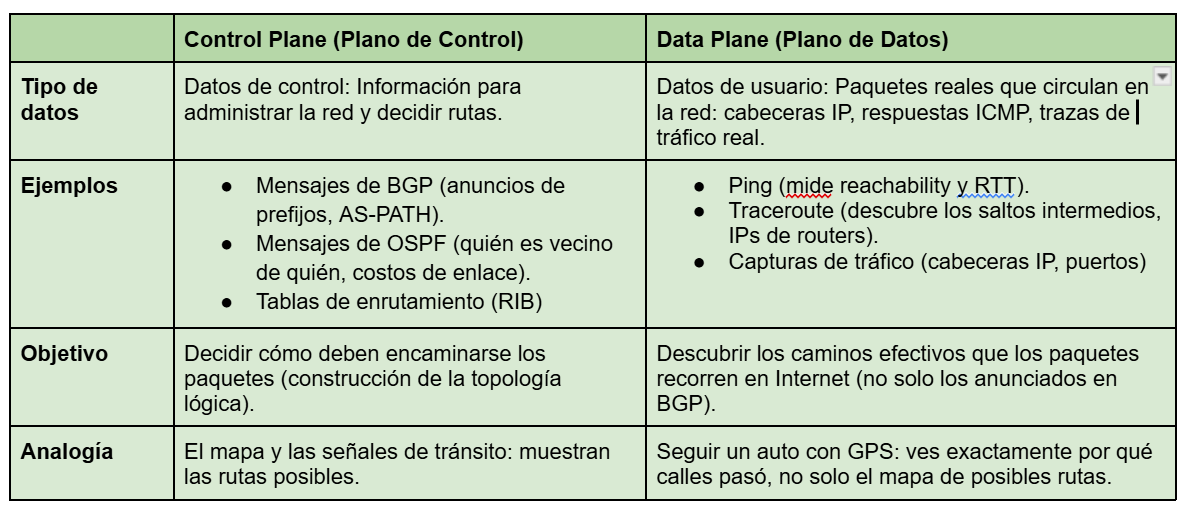
\includegraphics[width=0.9\textwidth]{Anexos/img/01/control_plane_vs_data_plane_tabla.png}
    \caption{Resumen conceptual de diferencias entre mediciones del plano de control y del plano de datos.}
    \label{fig:control_plane_vs_data_plane}
\end{figure}

En términos prácticos, BGP suele ofrecer un acceso escalable a rutas interdominio, mientras que \textit{traceroute} puede revelar enlaces que no aparecen en BGP (por ejemplo, enlaces en la periferia o enlaces que no son parte de la mejor ruta anunciada hacia un prefijo).

\subsection{Fuentes del plano de control: colectores BGP}

Los colectores BGP son infraestructuras públicas de recolección de información BGP diseñadas para observar el enrutamiento interdominio desde múltiples ubicaciones. En general, un colector establece sesiones BGP con distintos Sistemas Autónomos (los \textit{vantage points}) y almacena la información de enrutamiento que recibe.

Dos formas comunes de acceso a datos BGP son:
\begin{itemize}
    \item \textbf{RIBs (\textit{Routing Information Base})}: \textit{snapshots} periódicos de las tablas de enrutamiento observadas por el colector.
    \item \textbf{Updates}: mensajes incrementales que reflejan cambios en rutas (anuncios y retiros) y capturan parte de la dinámica del protocolo.
\end{itemize}

En este trabajo, las RIBs se usan como base para obtener rutas estables y construir la topología a nivel de AS. Los \textit{updates} pueden complementar este proceso cuando se desea observar variaciones temporales o rutas alternativas.

\subsection{Fuentes del plano de datos: medición activa}

Las mediciones del plano de datos, como \textit{traceroute}, permiten observar rutas a nivel de IP y, mediante técnicas de mapeo IP$\rightarrow$ASN, aproximar rutas a nivel de AS. Este tipo de medición presenta desafíos adicionales:
\begin{itemize}
    \item \textbf{Sesgo por puntos de medición}: la cobertura depende del número y ubicación de los \textit{vantage points}.
    \item \textbf{Aliasing y rutas asimétricas}: múltiples IP pueden corresponder a un mismo router y las rutas pueden diferir entre ida y vuelta.
    \item \textbf{Mapeo IP$\rightarrow$ASN}: no siempre es posible asignar cada salto IP a un ASN con certeza.
\end{itemize}

\subsection{Mapeo IP$\rightarrow$ASN}

Cuando se requiere transformar rutas IP a rutas AS, una estrategia común es el \textit{Longest Prefix Match}: a cada IP se le asigna el ASN del prefijo BGP más específico que la contiene, a partir de tablas de prefijos obtenidas de RIBs. Si un salto no puede mapearse (por ejemplo, por ausencia de prefijo o ambigüedad), se marca como desconocido o se omite el tramo según el criterio del análisis.

\subsection{Construcción del grafo a partir de datos BGP}

El objetivo es construir un grafo $G=(V,E)$ donde cada nodo $v \in V$ representa un Sistema Autónomo (ASN) y cada arista $e \in E$ representa adyacencias observadas entre ASes.

\subsubsection{Extracción de adyacencias desde \texttt{AS\_PATH}}

Sea una ruta BGP representada por una secuencia de ASNs:
\[
\texttt{AS\_PATH} = (a_1, a_2, \dots, a_k)
\]
Entonces se agregan adyacencias entre pares consecutivos:
\[
(a_1,a_2), (a_2,a_3), \dots, (a_{k-1},a_k)
\]
Dependiendo de la tarea, estas adyacencias pueden modelarse como aristas no dirigidas (para topología) o dirigidas (cuando se requiere asociar dirección a una relación).

\subsubsection{Limpieza de rutas}

Antes de construir el grafo, es habitual depurar rutas para evitar casos ambiguos o que introducen ruido. Por ejemplo:
\begin{itemize}
    \item descartar rutas con conjuntos de AS (AS-SET) u otras estructuras no lineales,
    \item remover duplicados consecutivos producto de \textit{prepending},
    \item descartar rutas con bucles evidentes,
    \item filtrar ASNs privados si aparecen en los datos.
\end{itemize}

\subsubsection{Ponderación y agregación de aristas}

Cuando una adyacencia aparece en múltiples rutas, se puede llevar un contador de ocurrencias y asociarlo como peso $w(u,v)$, lo que permite:
\begin{itemize}
    \item priorizar enlaces más observados,
    \item filtrar enlaces raros (posibles artefactos) usando umbrales,
    \item comparar estabilidad temporal del grafo entre diferentes fechas.
\end{itemize}

\subsubsection{Limitaciones}

Los grafos derivados de BGP reflejan alcanzabilidad y políticas del plano de control, pero no garantizan representar toda la conectividad física o contractual subyacente. Además, al observarse desde un conjunto limitado de \textit{vantage points}, existen sesgos y enlaces que no serán visibles (por ejemplo, enlaces de peering poco utilizados o rutas alternativas que nunca son seleccionadas como mejor ruta).
